% ------------------------------------------------------------------------------
% Chapter 2 : State of the Art
% ------------------------------------------------------------------------------
\setlength{\parindent}{4em}
\setlength{\parskip}{1em}
\section{What is Performance?}
Performance of any embedded system is depends upon the amount of the work accomplished by it and it depends upon many context. Performance depends upon many aspects. One of the aspect is response time, it is total time taken by system to respond the service being requested. Another aspect maybe processing speed, how many instructions are processed at a time provides the processing speed of the system. High throughput for input and output data, bandwidth, power consumption, latency, availability and many aspect are there for performance. In this thesis our main performance aspect is total number of cycles to execute the software at different phases.  


\par There are many techniques and tools are available to observe the performance of software on given embedded hardware. Some of these techniques are provided by tool vendors and some of them are part of industrial and educational research. Using tools provided by vendors, which helps to analyze the performance data graphically and provide more functionality and features to software engineers. Such tools are Silexica[link], ARM Streamline Performance Analyzer[link], or hardware simulation tools such as gem5 simulator[link to gem5]. Also there are ongoing research to evaluate the performance of software using machine learning techniques with state of the art. Using machine learning technique, it is possible to predict the performance of software by creating dataset of performance. Also using Worst Case Execution Techniques[WCET] use to analyze the performance.

	\par Traditional simulation approaches, simulator estimates the performance of software or application running on slow cycle accurate or cycle approximate models ISSs [1.3,2.7] of target embedded hardware processor. To improve the speed of ISSs and maintain the accuracy, hardware-assisted acceleration and transaction level techniques are recently proposed [2.5,2.8]. Chiang et al. [ieee] discusses the fast cycle accurate ISS for SoC based on QEMU and system C.  Li et. al[IEEE] discusses the inspection of problem to determine the WCET of processor. This paper further discuss issue of micro-architectural modeling to determine the WCET of known instruction sequence. Without need of source code or reverse engineering on binary files,it is possible to estimate WCET for software or application using integer linear programming(ILP) and constraint logic programming(CLP)[ieee]. Analytical model to estimate the performance of software on cross platform with using learning based techniques is discussed by Gerstlauer et. al [IEEE]. It evaluates the performance prediction of whole program using regression learning technique. Further they added new methodology[ieee] using learning model, to predict the power and performance of software at different phases of software or applications. Using analytical techniques, Joseph et.al [] obtains good approximate model Akaike's information criteria is used in iterative process to extract a linear model. Lee et al. [1.18] and Khan et al [1.14] focused on predictive modeling approach from uni-processor to multi-processor and multicore proccessor. 

\section{Analytical Models}
Analytical models are models which contains the information about behavior of system. It has data regarding input and output the system. Using this data which tell the behavior of system is used to form mathematical model or statistical model to understand the system. This analytical models are learned using learning algorithm techniques. There are different techniques to evaluate the performance of software on hardware by creating analytical models. Following are the state of the art performance analytical models used to predict the performance of software on processor.

\subsection{Learning-based Analytical Cross-Platform Performance Prediction}
This IEEE paper published by Gerstlauer and his colleagues from University of Texas at Austin, USA. This paper focuses about challenges with cycle accurate simulators and how analytical models is used to get performance evaluation of software at higher speed.

\par Simulation based models are widely used to model the hardware but these models are costly as well as slow to evaluate the performance of software using micro-architectural events. As collection of performance data on ISS is slow but collection of performance data on existing platform is faster because execution is done at native speed. Latent relationship can obtain by executing a program of processor and executing the same program of different processor. In this paper 'target' is preferred as platform for which the prediction is performed and 'host' is preferred as platform for which various statistics are collected. Host platforms are AMD Phenom II X6 1055T and Intel Core i7 Core. Target is platform is ARM processor model simulated on gem5 simulator.  

\par Performance of software on target and host platform is measured on single core using performance evaluation tool PAPI on each platform. PAPI measures all micro-architectural events from PMU with respect to software executing on hardware platforms. In this scenario, performance aspect is number of cycles consider. Total 157 programs with and 100 instances for each program are used to collect the training data. Input vector for Intel and AMD are different in term of number. Because number of performance counter supported by both processors are different. Intel i7 supports 14 where as AMD Phenom supports 8 hardware performance counter using PAPI. Training data collected from both host platform excepting the total cycles. total cycles event is collected on gem5 simulator for ARM processor for same 157 programs and 100 instances. Training data help to understand this relationship between input feature vector and output feature vector. Following figure \ref{fig:paper1} shows the framework for this paper. 

\begin{figure}[h!]
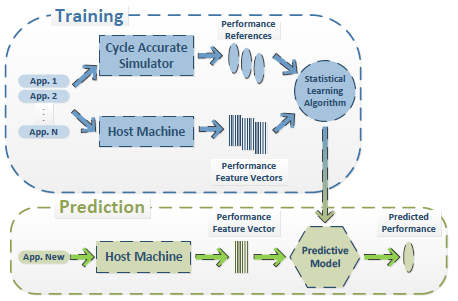
\includegraphics[width=12cm, height=8cm]{./images/ieee1}
\centering
\caption{Cross-platform performance prediction framework[]}
\label{fig:paper1}
\end{figure} 

\par To understand the collected training data, data is visualized using data analysis and data visualization techniques such as Principal Component Analysis(PCA) for reduce the dimensions and Co-relation coefficient for one to correlation of hardware performance counters. Using learning techniques this statistical model is learned and prediction is performed. Regression technique of machine learning is used. In which Lasso linear regression and Constrained Locally Sparse Linear Regression(CLSLR) are used. To select the best learning model cross-validation technique is used and as best result CLSLR is preferred. 

\par To test the accuracy of CLSLR algorithm,accuracy test is conducted on 15 different programs which are not used during training data collection. Input feature vectors for all these test programs are collected on both platforms. Result for predicting the whole program performance, errors of more than 40\% are observed on embedded benchmarks. 

\subsection{Accurate Phase-Level Cross-Platform Power and Performance Estimation}
This IEEE paper is also published by Gerstlauer and his colleagues from University of Texas at Austin, USA with improved and additional features with respect to previous paper. In this research, authors provided LACross method learning based method, for cross-platform time varying software performance as well power consumption predictions. Where all data is collected with fine-grained phase based approach. Also instead of simulation model, native hardware platforms are used for target and host.

\par In this approach host platform is Intel i7 920 processor used. Whereas as target platform, ODROID-U3[ref] development board is used which contains ARM Cortex-A9 processor and to collect the power consumption ODROID-XU3 development board is used with on-chip TI IN A231 current sensor. To collect training data, similar programs are used as it mentioned in previous paper except 100 instances, here only single instance is used. Training data collected on these hardware platform on single core using performance evaluation tool PAPI. Feature extraction for host platform contains all hardware performance counter except cycles where as feature extraction for target hardware are total cycles and power consumed. Following diagram illustrate the framework for LACross. It has similar goal is to accumulated latent relationship between to processor.

\begin{figure}[h!]
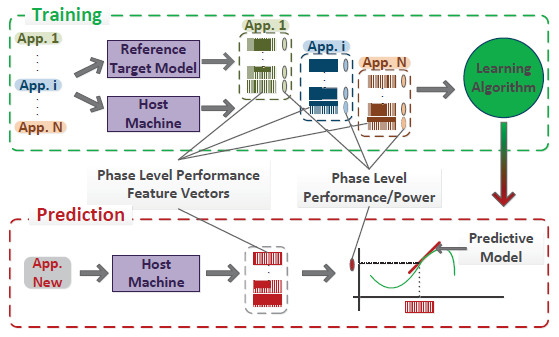
\includegraphics[width=12cm, height=8cm]{./images/ieee2}
\centering
\caption{LACross overview[]}
\label{fig:paper2}
\end{figure}

\par All these features are extracted using LLVM tool chain. Where LLVM uses Clang as compiler and it interfaced with PAPI libraries to collect the data at different phases of software. Time varying performance of software on hardware platform is collected in database. Values of performance counter is measured at each phase of software by inserting PAPI API calls to provide time varying data. 

\par All training data is gathered from host and target platform applied to learning algorithms. In this paper, variant of Lasso regression, that is Simplex Constrained Quadratic Programming(SCQP) applied to predict the performance and power consumption of software on hardware platforms at each phase level. All results are calculated on 
35 selected benchmark programs from three different standard benchmark suites. All these benchmark programs are not included during the training data collection phase. 
Results shows over average 97\% accuracy for both performance and power consumption at higher speed of 500 MIPS. 

\subsection{Composable Performance Regression for Scalable Multiprocessor Models}
This IEEE paper is published by Lee from Microsoft research in coopeartion with Intel and Harvard university with Collins,Wang, an Brooks respectively. Authors discuss about the regression model application to predict the performance on dual-core and quad-core multiprocessor using simulators. In uniprocessor simulators performance is estimated by tracking the resource utilization cycle whereas in multiprocessor simulators estimates th eperformance based on synchronization events and shared resources which increases the number of total cycles. In this paper authors propose Composable Performance Regression(CPR) method which directs to problems of multiprocessor simulation times by estimating the performance of of multiprocessor using combinations of uniprocessors, contention and penalty models. 

\par CPR uses composable models to predict the multiprocessor performance. Authors discus about uniprocessor model which is used in multiprocessor models. Uniprocessor model is basic building block of multiprocessor model. It uses uniprocessor regression model to reveal the accuracy of building block. Multiprocessor model uses CPR that contains the uniprocessor model, contention and penalty model, where uniprocessor model predict the performance of of each core, contention model predict the interfering accesses to shared resources from other cores. Penalty model contains the composed output of uniprocessor and contention model to produce final multiprocessor prediction. 

\par Total 18 benchmarks are used as workload to collect the training data on dual-core and quad-core. Using permutation and combination it provides 153 instances on dual-core and 3060 instances on quad-core processor. Simulation framework is based on IA-32 simulator. Uniprocessor training is performed using spline-based regression, contention training is also performed  using spline-based regression but on shares resource space and penalty training is performed using linear regression on full parameter. 

\par Prediction is performed for uniprocessor, contention and multiprocessor. 10 dual-core benchmarks and 20 quad-core benchmarks are used  for accuracy analysis. Dual-core models predicts the performance of each core with median errors of 6.63\% and quad-core models predict the performance of each core with median errors of 4.83\% across all benchmarks.

\section{WCET analysis}
\subsection{Combining instruction set simulation and WCET analysis for embedded software performance estimation}

\section{Silexica}
Silexica GmbH provides tools for software design automation which enables software developers and system architecture to design and program multicore systems via SLX tool suite. System architects work with software models which maybe open source, in house, commercial source, the traditional methods are not scalable for software optimization in multicore system. To understand the software or system behavior on multiocre system, a full and precise analysis of software interdependencies are required. So a tool is need to give deep insights on software interdependencies that occur during execution on multicore system. SLX is multicore development tool that provides software execution insights into hardware and software interdependencies.It allows for code architecting and refactoring to achieve the most efficient utilization of CPU, DSP, FPGA and other acceleration engines on multicore systems[].

\par SLX also can be use for software/hardware exploration. Current generation tools are not able to provide exploration to today's complex heterogeneous SoCs. These SoCs are big unimaginable challenges with present available tools. In current market of SoCs, SoCs with increasing number of cores, acceleration engine, decreasing the chip size are available in lower cost and high performance with less power consumption. In such wide varieties of SoCs, it is more challenging to fing optimal target platform for developing application. To select correct SoC for application requires clarity of software and hardware interaction. This interation can be useful to minimize disagreement and maz=ximize the performance. 

\par SLX features behavioral model for modeling multicore SoCs which made of co-processors, graphical processing units(GPUs), field programming gate arrays (FPGAs), communication buses, inter-connectivity, memory hierarchy and clusters. SLX system models provide rapid profile change with respect to hardware variance to facilitate hardware investigation for application software. SLX is able to predict the system behavior and memory performance based on simple and high level application model.

\par SLX analyze behvior of multiple application on target platform  and calculate the intercommunication delays. It also provides static and dynamic source code analysis, data and control dependencies. SLX also provide optimization to optimize the distribution of application to hardware and identification of blocking dependencies and control. Optimizations are driven by performance, power, and memory requirements for given combinations of FPGAs, GPUs and cores.  SLX support multiple programming languages to create high level application from scratch directly from your source code. It also support command line interface on windows and linux platforms. 

\par Silexica provides wide range of hardware platforms to analyze the behavioral of application software on different hardware platforms by measuring computing power, inter-connectivity, number of cores, delays and many more factors. It support software developers to understand the behavior of application on hardware platforms which may not be available in market or in still in prototype phase. 